\documentclass{article}
\usepackage{amsmath}
\usepackage{hyperref}
\usepackage{graphicx}
\usepackage{adjustbox}
\usepackage{caption}
\usepackage{subfigure}
\newcommand{\tabincell}[2]{\begin{tabular}{@{}#1@{}}#2\end{tabular}}
\begin{document} %This is where document begins
\begin{titlepage}
\title{EE 232E \\Graphs and Network Flows\\Homework 3\\Winter 2016} 
\author{Liqiang Yu, Rongjing Bai, Yunwen Zhu\\
904592975, 204587519, 104593417}  %change your ID here
\date{05-01-2016}
\end{titlepage}
\maketitle
\newpage
\tableofcontents
\newpage
\section{Problem 1}
After we construct the graph from the file, we found that the graph is not connected. The biggest connected component consists 10487 vertices out of 10501 vertices of the graph, however, there are 14 vertices belongs to other connected component.
\section{Problem 2}
For this directed graph, we collected the information about both in-degree and out-degree
\section{Problem 3}
When transforming the undirected network into directed network, it's not trivial to choose the method. Here we have two options : (1) we can keep the number of edges unchanged and just remove the direction, however it will lead to the  non-simple network. (2) or we can merge the two directed edges between two nodes and make the new weight the geometric mean of the original weight. The fast greedy method can only be applied to the second method and label propagation method can be applied to both.
\subsection{Option 1}
When using label propagation method to calculate the community structure for option 1, we got 5 communities, the sizes of each community are shown in table \ref{tb:p3_comsize}. From the table we can see that there is a dominant community with the size 10472, which means it cannot separate reasonable communities from the original giant connected component. The structure graph is shown in figure \ref{fig:lpc_opt1} and the modularity is $0.0001494257$.
\begin {table}[htbp]
\caption{The community sizes}
\begin{adjustbox}{center}
\label{tb:p3_comsize}
\begin{tabular}{|c|c|c|c|c|c|}
\hline
Index&1&2&3&4&5\\
\hline
Size&10472&4&5&3&3\\
\hline
\end{tabular}
\end{adjustbox}
\end{table}

\begin{figure}[htbp]
\centering
\captionsetup{justification=centering,margin=2cm}
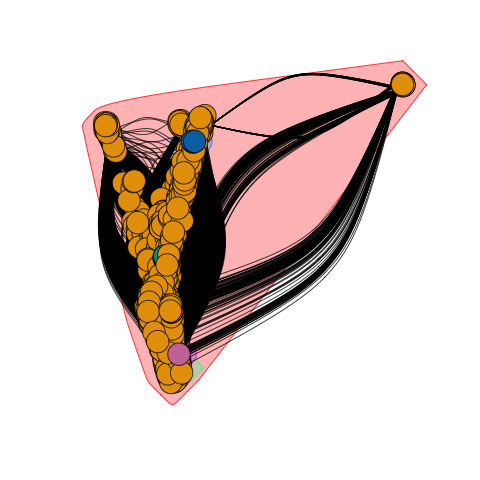
\includegraphics[width=.6\textwidth]{lpc_opt1.png}
\caption{The structure of the community derived from option 1 with label propagation method}
\label{fig:lpc_opt1}
\end{figure}

\subsection{Option 2}
We can use both label propagation method and fast greedy method to calculate the community for option 2. The respective community sizes are shown in table \ref{tb:p3_comsize_lpc} and table \ref{tb:p3_comsize_fgc}. 
The community structures are shown in figure \ref{fig:lpc_opt2} and figure \ref{fig:fgc_opt2}. The modularity for label propagation method is $0.0001698002$ and is $0.3287988$ for fast greedy method.
We can see that compared with label propagation method, fast greedy method will produce communities with more uniform sizes and higher modularity, which means the fast greedy method is more effective in this case.
\begin {table}[htbp]
\caption{The community sizes for label propagation method}
\begin{adjustbox}{center}
\label{tb:p3_comsize_lpc}
\begin{tabular}{|c|c|c|c|c|c|c|}
\hline
Index&1&2&3&4&5&6\\
\hline
Size&10469&4&5&3&3&3\\
\hline
\end{tabular}
\end{adjustbox}
\end{table}

\begin {table}[htbp]
\caption{The community sizes for fast greedy method}
\begin{adjustbox}{center}
\label{tb:p3_comsize_fgc}
\begin{tabular}{|c|c|c|c|c|c|c|c|c|}
\hline
Index&1&2&3&4&5&6&7&8\\
\hline
Size&1856&1666&1022&2266&731&1236&633&1077\\
\hline
\end{tabular}
\end{adjustbox}
\end{table}


\begin{figure}[htbp]
\centering
\captionsetup{justification=centering,margin=2cm}
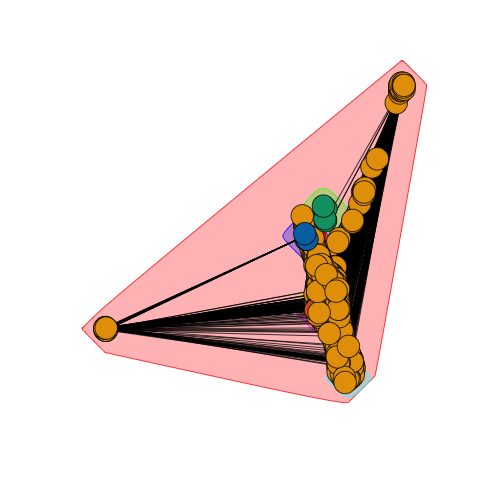
\includegraphics[width=.6\textwidth]{lpc_opt2.png}
\caption{The structure of the community derived from option 2 with label propagation method}
\label{fig:lpc_opt2}
\end{figure}

\begin{figure}[htbp]
\centering
\captionsetup{justification=centering,margin=2cm}
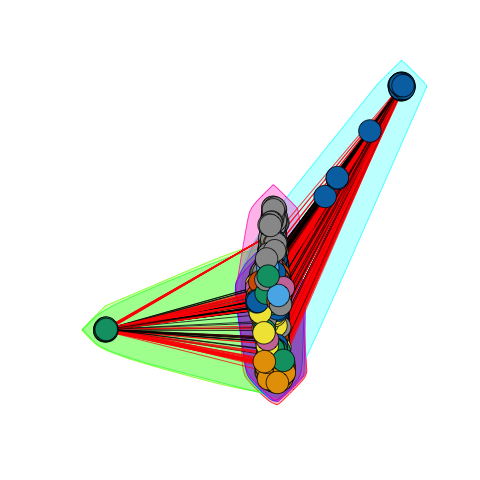
\includegraphics[width=.6\textwidth]{fgc_opt2.png}
\caption{The structure of the community derived from option 2 with fast greedy method}
\label{fig:fgc_opt2}
\end{figure}


\section{Problem 4}
We have calculated the communities with the fast greedy method in problem 3 and find that community 4 has the largest size of 2266. By deleting all the other nodes that don't belong to cummunity 4, we have another network. Then fast greedy method was applied on this network to calculate its structure. The sizes of community are shown in table \ref{tb:p4_comsize_fgc} and the structure graph is shown in figure \ref{fig:fgc_large}. The modularity is 0.3595153.

\begin {table}[htbp]
\caption{The community sizes for fast greedy method}
\begin{adjustbox}{center}
\label{tb:p4_comsize_fgc}
\begin{tabular}{|c|c|c|c|c|c|c|c|c|}
\hline
Index&1&2&3&4&5&6&7&8\\
\hline
Size&306&457&313&365&426&347&47&5\\
\hline
\end{tabular}
\end{adjustbox}
\end{table}

\begin{figure}[htbp]
\centering
%\captionsetup{justification=centering,margin=2cm}
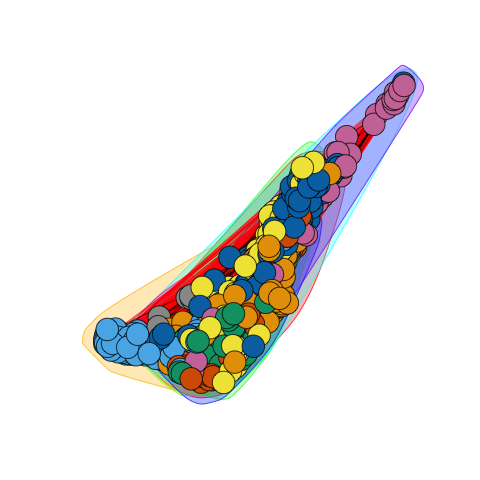
\includegraphics[width=.6\textwidth]{large_sub_com.png}
\caption{The structure of the largest sub community}
\label{fig:fgc_large}
\end{figure}

\section{Problem 5}
By deleting all the nodes which belong to the communities smaller than 100, we can calculate the structures of all sub communities which are larger than 100. From table \ref{tb:p4_comsize_fgc} we can see that there are six qualified communities and their modularities are shown in table \ref{tb:p4_subcom}. The structure graphs of all sub communities are shown in figure \ref{fig:all_sub}.

\begin {table}[htbp]
\caption{The modularity of all sub communities larger than 100}
\begin{adjustbox}{center}
\label{tb:p4_subcom}
\begin{tabular}{|c|c|c|c|c|c|c|c|c|}
\hline
Index&1&2&3&4&5&6\\
\hline
Modularity&0.372& 0.375& 0.433& 0.490& 0.474& 0.314\\
\hline
\end{tabular}
\end{adjustbox}
\end{table}

\begin{figure}[htbp]
\centering
\captionsetup{justification=centering,margin=2cm}

\subfigure{
\begin{minipage}[b]{0.4\textwidth}
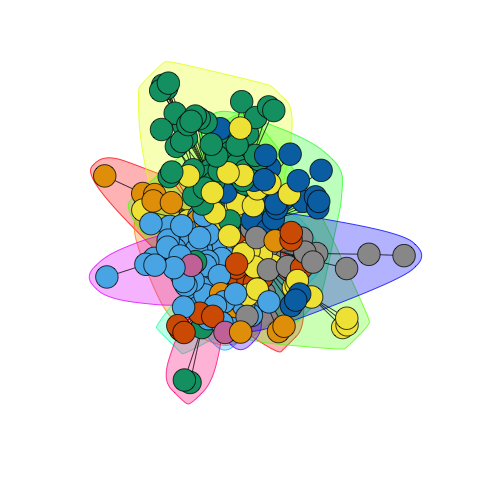
\includegraphics[width=1\textwidth]{sub_com_1.png} \\
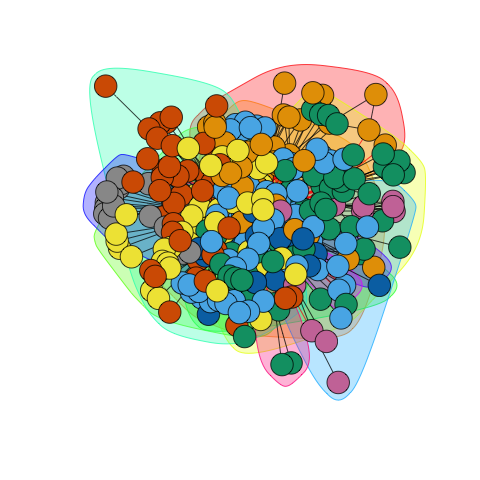
\includegraphics[width=1\textwidth]{sub_com_3.png}\\
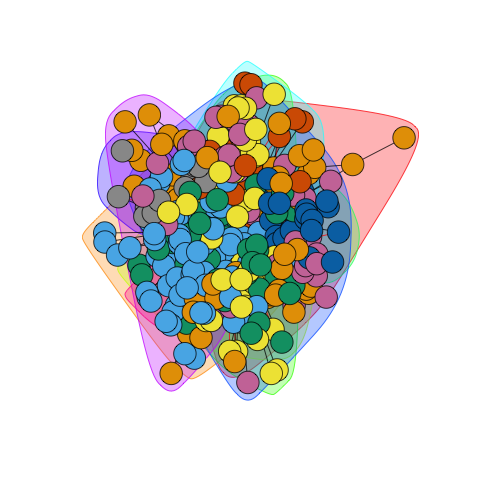
\includegraphics[width=1\textwidth]{sub_com_5.png}
\end{minipage}
}
\subfigure{
\begin{minipage}[b]{0.4\textwidth}
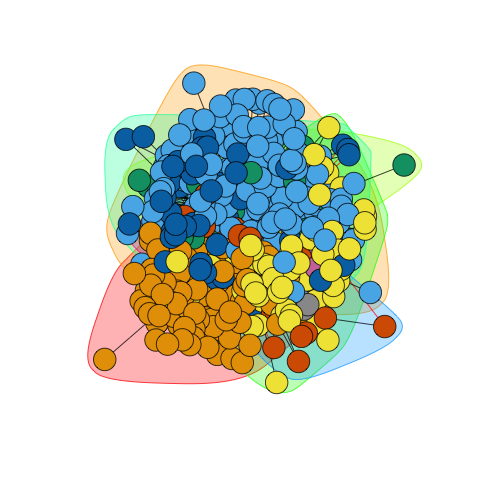
\includegraphics[width=1\textwidth]{sub_com_2.png} \\
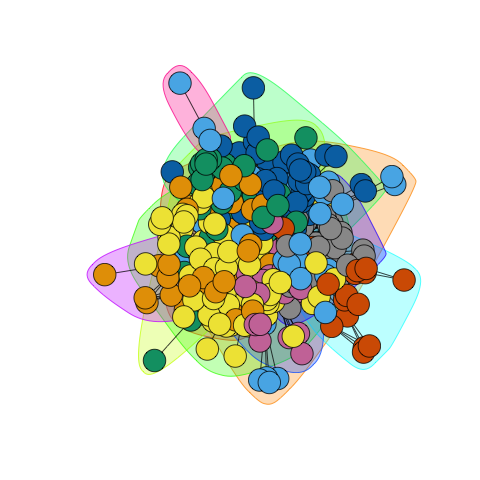
\includegraphics[width=1\textwidth]{sub_com_4.png}\\
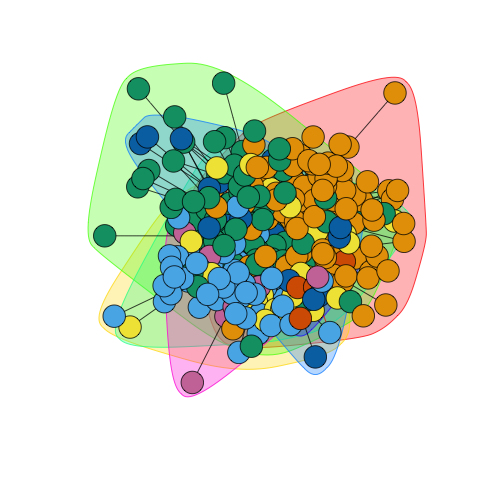
\includegraphics[width=1\textwidth]{sub_com_6.png}
\end{minipage}
}
\caption{The structure graphs of all sub communities with the size larger than 100}
\label{fig:all_sub}
\end{figure}

\section{Problem 6}
In order to study the strucutures of overlapped communities, we can use personalized pagerank. Every time we start a random walk from node $i$ with the damping parameter 0.85 in the original directed network, we can get the visit probabilities reflecting the relation between the other nodes and node $i$. Therefore we can compute\\
\begin{equation*}
\vec{M}_i=\sum_jv_j\vec{m}_j
\end{equation*}
\\
where $v_j$ is the visit probability of node $j$ and $\vec{m}_j$ is its community membership computed in Problem 3. In order to avoid the large amount of computation, we choose the largest 30 $v_j$ and replace values in $\vec{M}_i$ less than a specific threshold to zero.\\
\\
It is tricky to find a proper threshold. Here we plot the distribution of the largest values and the second largest values of $\vec{M}_i$ in figure \ref{fig:p6_dist}. From the histograms we can see that if we choose a small threshold there will be too many nodes belonging to multiple communities, however if we choose a large threshold there will be some nodes belonging to no community. So there is a tradeoff. Since the problem asked us to detect at least three nodes, we choose a relative large threshold 0.024 and hince found 11 nodes belonging to multiple communities, their indices are 375, 385, 389, 3629, 5808, 6631, 6634, 6635, 6650, 9608, 9942.

\begin{figure}[htbp]
\centering
\captionsetup{justification=centering,margin=2cm}

\subfigure[The distribution of the largest values]{
\begin{minipage}[b]{0.4\textwidth}
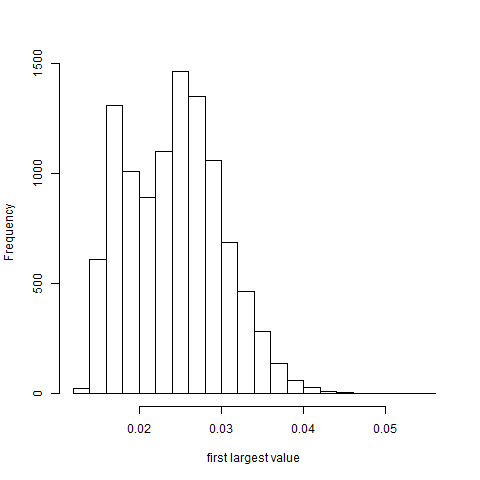
\includegraphics[width=1\textwidth]{dist_firstlarge.png}
\end{minipage}
}
\subfigure[The distribution of the second largest values]{
\begin{minipage}[b]{0.4\textwidth}
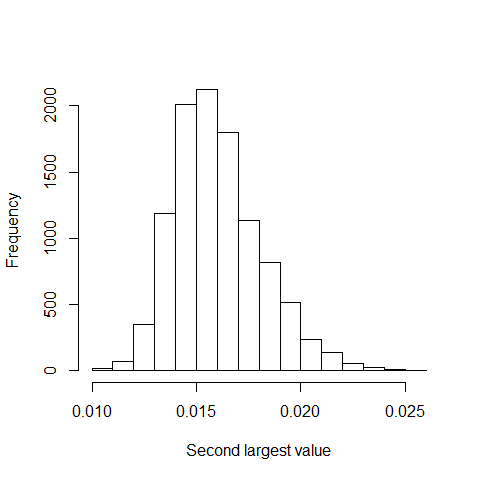
\includegraphics[width=1\textwidth]{dist_secondlarge.png}
\end{minipage}
}
\caption{}
\label{fig:p6_dist}
\end{figure} 
\end{document}
